\section{面向开放组织的数据信息挖掘框架}
% 从Github全域数据中能提取到什么信息,即看板展现的内容。【数据结构】(这里要直接讲数据结构吗?】
% 意义:
% 快速挖掘出项目中的深层信息
% 帮助开源项目的管理
% 帮助个人职业规划与发展
% \par 上一章中,对开源社区中开放数据的探索性分析从社区活跃情况、开源开发者的工作时间分布、开发语言的使用、项目或开发者之间的协同关系四个角度,带来了对项目或个人开发者行为的更深层解读,揭露了开源社区庞大的开放数据中所含信息量的冰山一角。如果这些信息能够被快速挖掘、定向展现,那么将大大助益开源社区的发展。

\par 对于开源开发者而言,通过个人行为数据的汇总挖掘,能够更好地自我了解与进行职业规划;对于开源项目而言,这些数据将提供不同的维度来评估其影响力、国际化程度,即便对于项目不熟悉的人,也能在很短的时间内快速了解项目状况,更可以方便项目管理与社区治理\cite{kalliamvakou2014promises}。


% \subsection{衡量指标定义}
% 活跃仓库与开发者统计方法;
% ​开发者活跃度;
% ​项目活跃度;
% 时区估计方法;
% 主要开发语言;
% ​开发者协作网络构建方法;
\subsection{活跃仓库与开发者统计方法}
\par 若被统计的代码仓库包含事件日志,仓库即被定义为活跃仓库;若开发者有任意代码仓库包含事件日志,开发者即被定义为活跃开发者。

\subsection{开发者活跃度}
\par 开发者活跃度,其定义为某特定 GitHub 账号在一段时间内在某特定 GitHub 项目中的活跃评价指标。其活跃度由该账号在该项目中的行为数据决定,本文中所关心的行为包含如下几种:\cite{王伟2020全球开源生态发展现状研究}

\begin{itemize}
    \item Issue comment:在 issue 中参与讨论是最基本的行为,每个评论计入 1 次。
    \item Open issue:在项目中发起一个 issue,无论是讨论、bug 报告或提问,对项目都是带来活跃的,每个发起的 issue 计入 1 次。
    \item Open pull request:为项目提交一个 PR,表示已对该项目进行源码贡献,则每次发起一个 PR 计入 1 次。
    \item Pull request review comment:对项目中的 PR 进行 review 和讨论,需要对项目有相当的了解,并且对项目源码的质量有极大帮助,每个评论计入 1 次\\
          注:仅通过代码 review 对特定代码行的讨论记为 review,直接对 PR 的评论回复记为 issue comment 事件。
    \item Pull request merged:若有 PR 被项目合入,即便是很小的改动,也需要对项目有较为深入的理解,是帮助项目进步的真切贡献,则每有一个 PR 被合入计入 1 次,同时 PR 合入事件根据该 PR 的代码增加行数。
    \item Watch:用户 star 项目,被计入 1 次。注:Star 操作在 GitHub 日志事件中记为 Watch 事件。
    \item Fork:开发者 fork 该项目,被计入 1 次。
\end{itemize}

以上 7 个种行为各自独立计数,具有不一样的权重,根据专家经验,加权值分别为 1、2、3、4、2,1,2,即:
$$
 A_{u\_d}=C_{issue\_comment}+2{C}_{open\_issue}+3{C}_{open\_pr}+4{C}_{review\_comment}+2{C}_{pr\_merged}+{C}_{watch}+2{C}_{fork} 
$$
其中,Pull request merged 的计数由分段函数决定\cite{tsay2014influence}:

$$ C_{pr\_merged}=\left\{
    \begin{array}{rcl}
        0.8+0.002 \times loc &  & {loc < 100}          \\
        1                    &  & {100 \leq loc < 300} \\
        2.5-0.005 \times loc &  & {300 \leq loc < 400} \\
        0.5                  &  & {loc \geq 400}
    \end{array} \right.
$$

其中,loc 表示新增的代码行数。根据软件计量学经典数据统计,单次代码变更最佳在 200 行以内,超过 400 行的代码变更会导致审阅困难,故通过分段函数关联了代码新增行数与 PR 的权重指标。

\subsection{项目活跃度}
\par 项目活跃度定义为某特定项目在一段时间内的活跃评价指标。其活跃度由单开发者在一天内的活跃度加总计算得到(时间点与时间段计算方式均基于开发者个人活跃度方式计算):

$$ A_{r} = \sum (A_{u\_d} / day\_count) $$

开发者活跃仓库数量,则在此基础上定义为,由每个开发者所产生的活跃度大于 0 的仓库数量。

\subsection{开发者时区估计方法}

\par 根据开发者全年每小时产生日志的数量,计算获取其事件最多的连续 12 个小时,令其时间为该开发者本地时间的 9 时至 21 时,则可以大致确定该开发者的所属时区。因为日志所记录的时间为 UTC 标准时间\footnote{
UTC 即协调世界时间,是国际通用的时间标准,将全球各地的时间进行同步协调。UTC 时间是经过平均太阳时(以格林威治时间 GMT 为准)、地轴运动修正后的新时标以及以秒为单位的国际原子时进行综合精算而得到的。
世界时区使用 UTC 的正或负偏移量表示。最西端的时区使用 UTC-12,比UTC落后十二小时;最东部的时区使用 UTC+14,比 UTC 早 14 小时。出现 UTC+13,UTC+14 的原因如下:
    \begin{enumerate}
        \item[1)] 因为国际日期变更线,虽然1884年划定时避免在一个国家中同时存在着两种日期,但是1979年成立的基里巴斯领土却跨越了国际日期变更线。基里巴斯的UTC有:莱恩群岛(UTC+14)、菲尼克斯群岛(UTC+13)、吉尔伯特群岛(UTC+12),这样保证一个国家内的日期为同一天。
        \item[2)] 因为夏令时,即天亮早的夏季人为将时间调快一小时。比如新西兰是 UTC+12,在夏时制改用 UTC+13。
    \end{enumerate}
北京时间是中国采用国际时区东八时区的区时作为标准时间,东八区(UTC+8)是比 UTC 早 8 小时的时区。
}。考虑开发者一天连续 12 个小时产生日志数最多的最后一个小时,其最后一小时(即本地时间 21 时)对应的 UTC 时间记为 $ k $, 则时区计算公式如下:
$$
    zone=
    \begin{cases}
        20-k^*, & k^*>8 \quad \text{对应本地为东时区}     \\
        -4-k^*, & k^*\le 8  \quad \text{对应本地为西时区}
    \end{cases}
$$

\par 其中,数学公式: $ k^*=argmax\{\sum_{i=k-11}^{k}{c_i} \},\quad  k=0,1,...,23 $, $ c_i $表示当前小时产生的日志数量。当 i 为负值时,意味着为前一天的时间,需进行转换,即使用数学公式: $ i=i+24 $进行转换。

\par 因单个开发者的行为具有偶发性与特殊性,本方法不可用于单开发者时区的精确估计,但其在统计维度上具有意义,在此仅考虑统计学意义。再者,活跃度较低的开发者,其行为发生也具有偶发特性,所以在对开发者时区判断时,剔除了 GitHub Apps 并只保留全域活跃度排名前 5 万名的开发者账号用于分析,得到的工作时间画像如图2-3所示。

\begin{figure}[H]
    \centering
    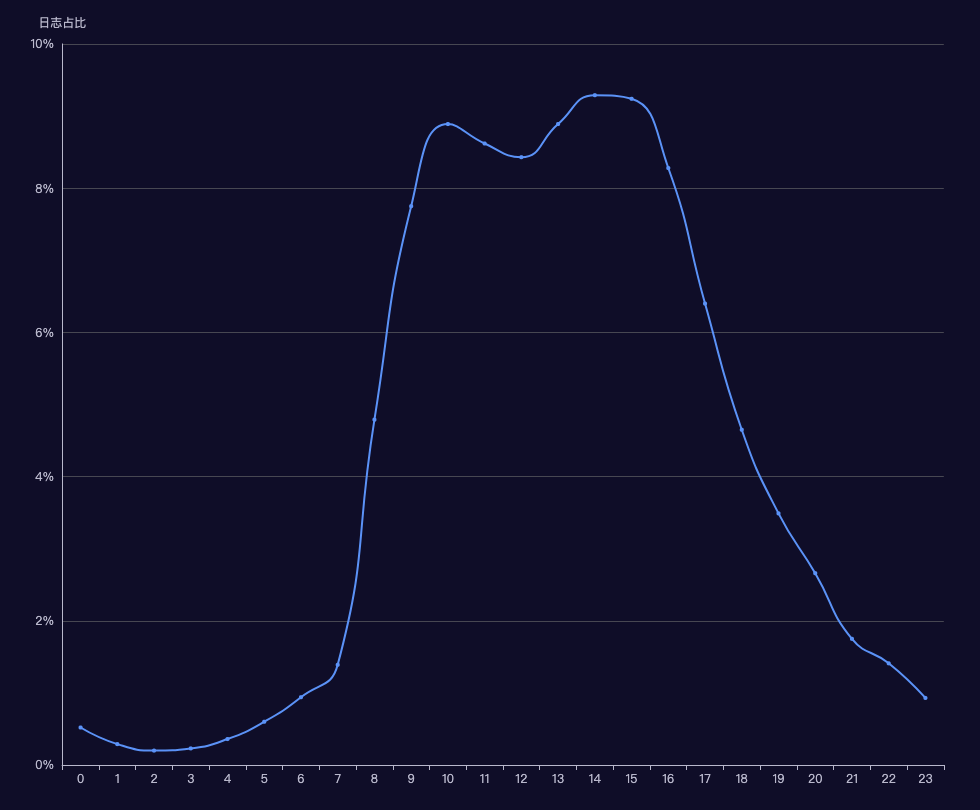
\includegraphics[width=130mm]{./figures/image2-3.png}
    \caption{ 典型开源开发者工作时间画像\\Figure 2-1: Portrait of a typical open source developer's working hours}
\end{figure}

\par 由图2-3所示,开发者通常会选择从当地时间早上 8 时开始工作,中午 11 - 13 时进行短暂的午休,随后在下午 15 - 16 时达到一个生产力高峰,并持续产出到晚间,较符合常见的工作时间情况;另一方面,可以看到开发者在晚间的工作产出比例还是较高的,甚至可以工作到凌晨 1 点,活跃程度应该明显高于一般职业。

\par 在高活跃开发者中,UTC-8 至 UTC-3,即美洲(美国、加拿大、南美)开发者分布最多,虽然单时区的开发者比例不是最高,但总体开发者占比高达 33\% 左右。而 UTC+1 至 UTC+3,即欧洲拥有最高的单时区开发者比例,UTC+1 时区高达近 10\%,三个时区的总占比约为 26\% 左右。总体而言,亚洲的开发者数量依然较少,但在 UTC+7 至 UTC+8 区域有一个小的波峰,说明中国、俄罗斯开发者相较其他国家还是有较高的开源活跃。而太平洋地区(UTC+9 至 UTC-9)则由于人口分布原因,开发者比例最低。


\subsection{开发者使用语言统计方法}
\par 开发者使用语言定义为一个开发者账号在该年度使用频率最高的语言,其具体实现为一个开发者账号在该年度提交并合入 PR 最多的项目所使用的主要编程语言。


\subsection{​开发者协作网络构建方法}
开发者协作网络是基于上文中开发者活跃度的定义,通过多个开发者在项目中的协作关系进行构建的。具体计算方式为:

$$ R_{ab}=\sum_{i}{\frac{A_{ia}A_{ib}}{A_{ia}+A_{ib}}} $$

其中 $ A_{ia}, A_{ib} $分别为开发者i在项目 a 和项目 b 上的活跃度,计算方法遵循2.2中的计算方法。 $ R_{ab} $为项目 a 和 项目b 的协作关联度。即两个项目的协作关联度为其所有共同活跃开发者的活跃度的调和平均值之和。

\subsection{项目协作网络构建方法}
项目协作网络是基于上文中项目活跃度的定义,对具有共同开发者的项目的进行构建。具体构建过程为将每个开发者的全年活跃度计算精细化到具体的 issue/PR 之上,则同时在同一个 issue/PR 上有过活跃的开发者认为其具有协作关系,而协作关系与两人在该 issue/PR 上的活跃度相关,具体计算方式为:

$$ R_{ab}=\sum_{i}{\frac{A_{ia}A_{ib}}{A_{ia}+A_{ib}}} $$

其中 $ A_{ia}, A_{ib} $分别为开发者 a 和 b 在 issue/PR i 上的活跃度,计算方法遵循开发者活跃度计算方法, $ R_{ab} $为开发者 a 和 b 在该项目上的协作关联度。即两个开发者在项目的协作关联度为其在所有共同活跃的 issue/PR 上的活跃度的调和平均值之和。

\subsection{开源象限分析}
\par 提出一种开源象限(OpenQuadrant)的方法来刻画一个开源项目在影响力、全球化、社区规模三个核心特性方面的表现。基于该开源象限分析,使用散点图来表示,横纵两个维度为项目影响力指标和项目全球化指标,为了方便可视化,我们采用取对数的形式呈现上述两个指标,而使用散点图上的点的大小来刻画项目参与的活跃人数,用来反映一个项目的社区规模。\cite{vasilescu2015quality}

\par 以2020年CNCF基金会( Cloud Native Computing Foundation,即“云原生计算基金会”)下云原生领域的开源象限分析结果为例,如图2-2所示,
\begin{figure}[H]
    \centering
    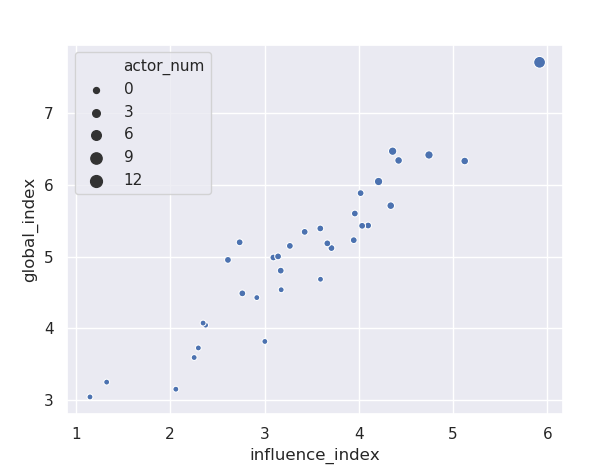
\includegraphics[width=100mm]{./figures/开源象限.png}
    \caption{CNCF 下云原生领域的开源象限\\Figure 2-2: Open source quadrant in the cloud native field under CNCF}
\end{figure}
基于以上,开源象限将整个平面分成了四块区域,分别是:
\begin{itemize}
    \item 前瞻(Foresighted):落在该区域的项目影响力强,同时项目全球化程度高;
    \item 引领(Leading):落在该区域的项目影响力强,但项目全球化程度较低;
    \item 行动(Acting):落在该区域的项目影响力较弱,但项目全球化程度高;
    \item 进入(Incubating):落在该区域的项目影响力较弱、同时项目全球化程度也较低。
\end{itemize}
\par 影响力、全球化、参与人数的具体计算方式如下所示。

\subsubsection{领域项目影响力指标}
% //TODO:领域项目影响力指标的定义
\par 基于项目协作网络构建方法,得到全域活跃项目数105.7万,协作关系共计2,607万个节点、2,607万条边的无向图。在该图上应用加权PageRank算法至收敛(共计迭代128次),得到每个结点的PageRank值为该节点影响力指标。

\subsubsection{领域项目全球化指标}
\par 全球化的影响因素众多,考虑地域、开发者人数这两个因素用于项目全球化指标的计算。针对地域因素,考虑计算参与该项目的开发者的时区分布情况,开发者时区分布趋于均匀分布,即标准差越小时,认为该项目的全球化程度越高。因此,首先通过判断项目上所有开发者的时区,之后计算了项目在 24 个时区上对应的开发者人数,在此基础上,计算项目关于时区人数的标准差。针对开发者人数因素,即该项目上参与的开发者总数,开发者人数越多,该项目全球化程度越高。考虑到开发者人数不多,但开发者的行为具有偶发特性的情况,该情况导致地域因素计算不准确,从而导致全球化指标的结果不准确。因此,使用如下全球化指标计算公式:

$$ \sqrt{\frac{24}{\sum_{i=-12}^{11}{(x_i-\bar{x})^2}}}\bar{x}^2, \quad x_i\text{表示该项目在i时区的开发者人数。} $$

\par 上述计算公式表明,全球化指标与项目时区开发者人数均值的平方成正比,与项目时区开发者人数的标准差成反比。该计算方式能够有效评估开发者人数较少的项目的全球化程度,另一方面,该计算方式对开发者人数较多的项目,全球化指标计算有正向作用。

\subsection{项目参与人数}
\par 项目参与人数,即在项目上发生日志行为的参与者总数。在可视化散点图点的处理上,我们对领域项目的参与人数使用线性最大最小归一化,使得数值映射到了1-10区间范围内\cite{mcdonald2013performance}。


% \subsection{数据设计}
% \subsection{开发者分析方法}
% \par 以某开发者数据为例,取半年作为时间区间,设计如下图表:

% \subsubsection{个人活动}
% % 开发者活跃度-折线图
% % 工作时间分布-打孔图
% % Github事件雷达图
% \paragraph{开发者活跃度} 以时间为横坐标,以开发者活跃度为纵坐标,展示形式为折线图。

% \paragraph{工作时间分布} 横轴为一天 24 个小时(UTC标准时间),纵轴为一周 7 天,圆点大小表示该时段产生的日志量的相对大小。

% \paragraph{事件雷达图} 以该开发者的Star、Fork、Commit、OpenIssue、OpenPR、PR review事件次数作雷达图。

% \subsubsection{个人发展}
% % 语言使用分布-百分比堆积条形图
% % 个人关注点-Issue label词云
% \paragraph{语言使用分布} 将用户的各项目仓库中占比最大的语言作为该项目的开发语言,统计用户所有项目语言种类,并计算占比,以百分比堆积条形图的形式呈现。

% \paragraph{个人关注点} 在开放平台的issue板块,用issue做任务划分和bug记录时,项目管理人员或issue的发起者常常使用标签来给issue做标注,以便于区分issue类型,这种标签便被称为issue label。统计个人开发者参与或发起的issue所带issue label,按出现频率生成词云,能够展现该开发者在开发过程中的个人关注点。

% \subsubsection{协作关系}
% % 开发者协作-网络图
% % 项目关联-网络图
% \paragraph{开发者协作网络} 凡是与某开发者之间协作活跃度$R_{ab} > 0$ 的开发者,取top N位(N由用户定义配置)生成网络图,图中节点描述各开发者,节点大小描述开发者活跃度,节点之间边的粗细描述协作活跃度。支持交互式访问,点击节点跳转至协作者的主页。

% \paragraph{关联项目网络} 在开发者作出commit、PR贡献的所有项目中,取top N个项目(N由用户定义配置)生成网络图,图中节点描述各项目,节点大小描述用户对该项目的贡献量。
% % TODO: 贡献怎么定义的?节点间有无连接?
% % 贡献量:开发者对项目所作出的活跃度的贡献,开发者在这个项目的活跃度/项目活跃度

% \subsection{项目分析方法}
% \par 以某项目数据为例,取半年作为时间区间,设计如下图表:
% \subsubsection{项目生命力}
% % 活跃度-曲线图
% % 一周commits、star、fork-复合曲线
% % 参与度
% %   打开/关闭的issue-双向柱状图
% %   代码行数变化-双向曲线图
% % 项目回应度基于每日issue和pr的初次响应时间
% %   PR平均解决周期(每月)-热力图
% %   Issue平均响应时间-?
% \paragraph{项目活跃度} 以时间为横坐标,以项目活跃度为纵坐标,展示形式为折线图。在此基础上复合以每周commit、star、fork数量为纵坐标的堆叠折线图。
% \paragraph{issue状态} 以周数为横轴,以每周的issue数量为纵轴,向纵轴的正、负方向分别作打开、关闭状态issue的双向柱状图。
% \paragraph{代码行数变化} 以时间为横轴,以每天的代码量增减行数作为纵轴,向纵轴的正、负方向分别作代码增加、减少行数的双向曲线图。
% \paragraph{PR平均解决周期} 
% % TODO: 纵轴是什么
% \paragraph{Issue平均响应时间} 


% \subsubsection{项目多元化}
% % 参与人数与New Contributer的数量-百分比堆积条形图
% % 工作时间分布-打孔图
% % 开发者时区分布-柱状图
% \paragraph{参与人数与New Contributer的数量} 定义最近一周内参与贡献的开发者为该项目的New Contributer,统计项目所有的参与人数与New Contributer数量,并计算占比,以百分比堆积条形图的形式呈现。
% \paragraph{工作时间分布} 根据事件日志的时间戳作打孔图,横轴为一天 24 个小时(UTC标准时间),纵轴为一周 7 天,圆点大小表示该时段项目内产生的日志量的总和。
% \paragraph{开发者时区分布图} 对项目内部所有开发者进行时区估计,随后以UTC标准时间下的24个时区为横轴,以每个时区开发者比例为纵轴,作分布直方图。

% \subsubsection{协作的力量}
% % 开发者协作-网络图
% % 关联项目-网络图
% % 一周活跃开发者榜单(top N)-List
% % 开发者留存率-?
% \paragraph{开发者协作网络} 对于在该项目中作出贡献的开发者,取top N位(N由用户定义配置)生成网络图,图中节点描述各开发者,节点大小描述开发者对该项目的贡献量,节点之间边的粗细描述两个开发者之间的协作活跃度。支持交互式访问,点击节点跳转至协作者的主页。

% \paragraph{关联项目网络} 对于参与该项目的开发者作出commit、PR贡献的其他项目,生成网络图,图中节点描述各项目,节点大小描述项目活跃度,节点之间边的粗细描述项目之间的相关性。
% % TODO: 项目间的相关性是怎么定义的?
% \paragraph{一周活跃开发者榜单} 在本周活跃开发者中取top N(N由用户定义配置)个,按贡献度顺序形成列表。列表包含开发者id与贡献度。


% \subsection{社区分析方法}
% \par 上文中对于项目的分析方法也同样适用于社区分析,唯一的不同在于社区分析的数据来源于社区组织下所有项目的事件日志总和。在此基础上,再对社区分析增加以下方法。
% \subsubsection{开源象限分析}
% % 影响力、全球化、社区规模
% 提出一种开源象限(OpenQuadrant)的方法来刻画一个开源项目在影响力、全球化、社区规模三个核心特性方面的表现。基于该开源象限分析,使用散点图来表示,横纵两个维度为项目影响力指标和项目全球化指标,为了方便可视化,我们采用取对数的形式呈现上述两个指标,而使用散点图上的点的大小来刻画项目参与的活跃人数,用来反映一个项目的社区规模。

% 基于以上,开源象限将整个平面分成了四块区域,分别是:
% \begin{itemize}
%     \item 前瞻(Foresighted):落在该区域的项目影响力强,同时项目全球化程度高;
%     \item 引领(Leading):落在该区域的项目影响力强,但项目全球化程度较低;
%     \item 行动(Acting):落在该区域的项目影响力较弱,但项目全球化程度高;
%     \item 进入(Incubating):落在该区域的项目影响力较弱、同时项目全球化程度也较低。
% \end{itemize}




